\documentclass[aspectratio=169]{beamer} 
\usetheme{UASLP1}
\usepackage[utf8]{inputenc}
\usepackage[T1]{fontenc}
\usepackage{media9}
%% Use any fonts you like.
\usepackage{helvet}

\title{Using Culturally Relevant Game Based Education Strategy}
%\subtitle{Presentations in Latex Beamer}
\author{Anuroop Gaddam }
\date{ \today}
\institute{School of Engineering \& Computer Science \\
Victoria University of Wellington, New Zealand\\
\url{Anuroop.Gaddam@vuw.ac.nz}}

\begin{document}

\begin{frame}[plain,t]
\titlepage
\end{frame}


\section{Introduction}
\begin{frame}
\frametitle{Introduction}
%\framesubtitle{Bullet points}
\begin{itemize}
\item Computer science education is increasingly becoming a compulsory part of schooling
	\newline
\item Within the New Zealand (NZ) context, there is the unique challenge of providing relevant teaching material and learning experiences for children with a M\=aori and Pasifika background.
	\newline
\item Currently, M\=aori and Pasifika students are an underrepresented group in computer science engineering in universities across NZ
\end{itemize}
\end{frame}

\section{Research Questions}
\begin{frame}
\frametitle{Research Questions}
\begin{itemize}
\item How to encourage and increase active participation of M\=aori \& Pasifika students who are considered as the underrepresented group in computer science engineering
	\newline
\item How to engage these students to effectively learn computer science concepts in a way that is culturally relevant
	\newline
\item Instead of teaching computer science from a traditional (i.e. western) viewpoint, can we consider and utilize the learner’s \textbf{values, cultural setting} and \textbf{perspectives} to develop modern interactive learning approach
	
\end{itemize}
\end{frame}



\subsection{Aim}
\begin{frame}
\frametitle{Aim}
\textit{\textbf{The aim is to integrate the teaching and learning with cultural concepts to enable learning computer science concepts}} 
\begin{figure}
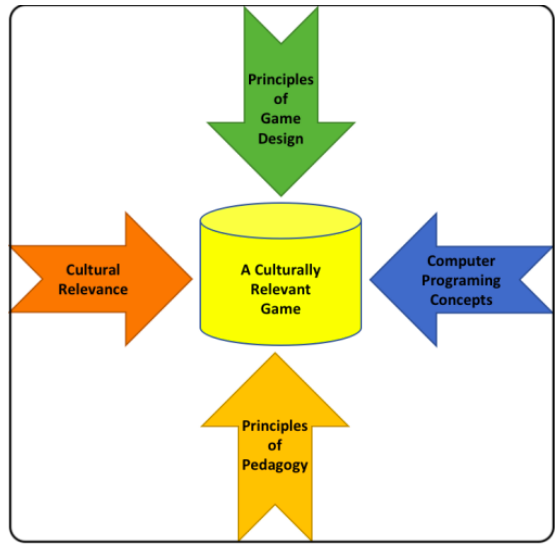
\includegraphics[scale=0.24]{p1.png}
\end{figure}
\end{frame}

\section{Our Approach}
\begin{frame}
\frametitle{Our Approach}
\begin{itemize}
\item The goal of the research is to create an educational game that teaches programming concepts using \textbf{te reo M\=aori} \textit{(the language of the M\=aori people)} commands  as a \textbf{simple programming language} within the game
\newline
\item We designed a game design-based method to teach key computer science concepts called \textit{Te Ika-a-Māui}
\newline	
\item The game is designed to teach key computer science concepts through using everyday commands in te reo M\=aori using a Maori story 
	
\end{itemize}
\end{frame}

\section{The Game}
\begin{frame}
\frametitle{Te Ika-a-Māui}
\framesubtitle{The Game Storyline}
\begin{itemize}
\item  A game based around a Maori character called “Kupe” was developed. 
\newline
\item According to the narrative, Kupe was involved in the Polynesian discovery of New Zealand.
\newline	
\item He had problems with a great octopus – “Te Wheke-a-Muturangi” belonging to Kupe's competitor - “Muturangi”.  
\newline	
\item On a quest to kill the octopus, the length of the pursuit brings him to New
Zealand. 	
\end{itemize}
\end{frame}
\subsection{Storyline}
\begin{frame}
\frametitle{The Game Storyline}
Screen-shots of the Mobile Games
\begin{columns}[t]
\column{.5\textwidth}
\centering
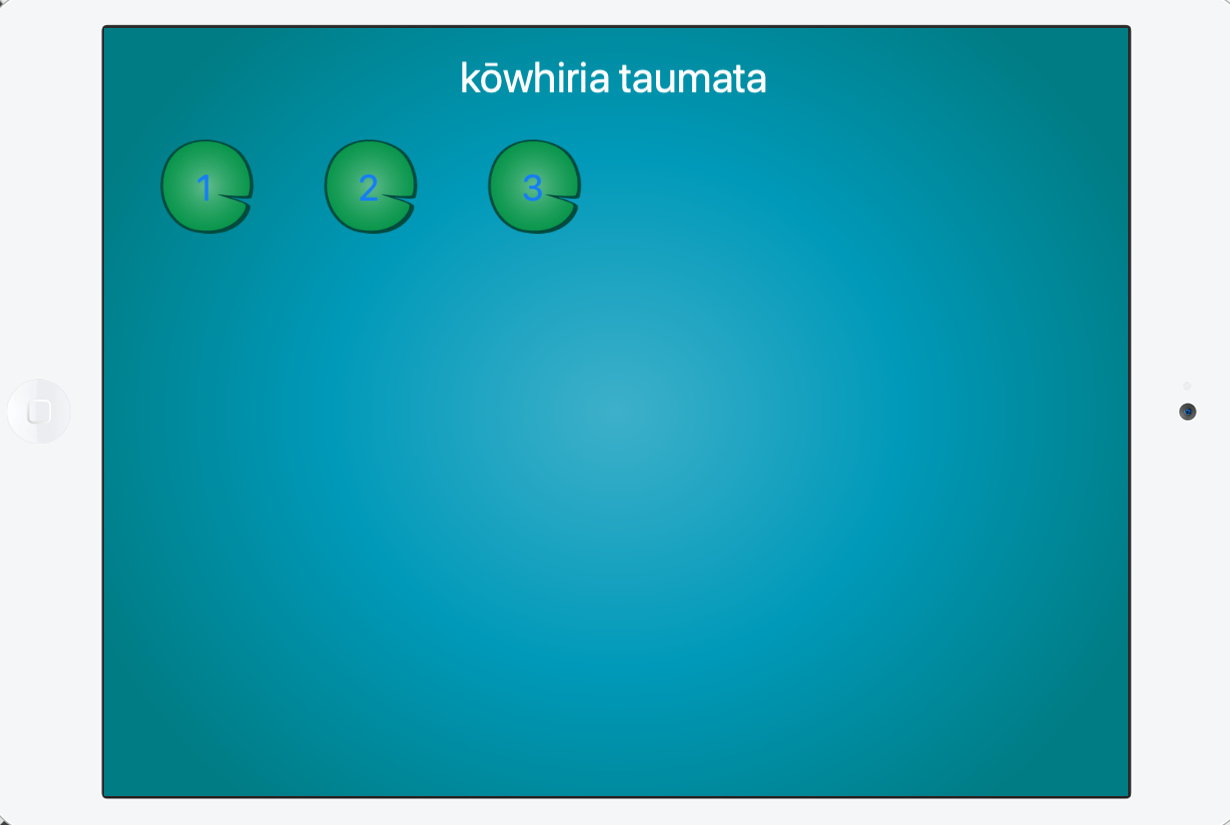
\includegraphics[width=5cm,height=3.5cm]{p2.png}\\
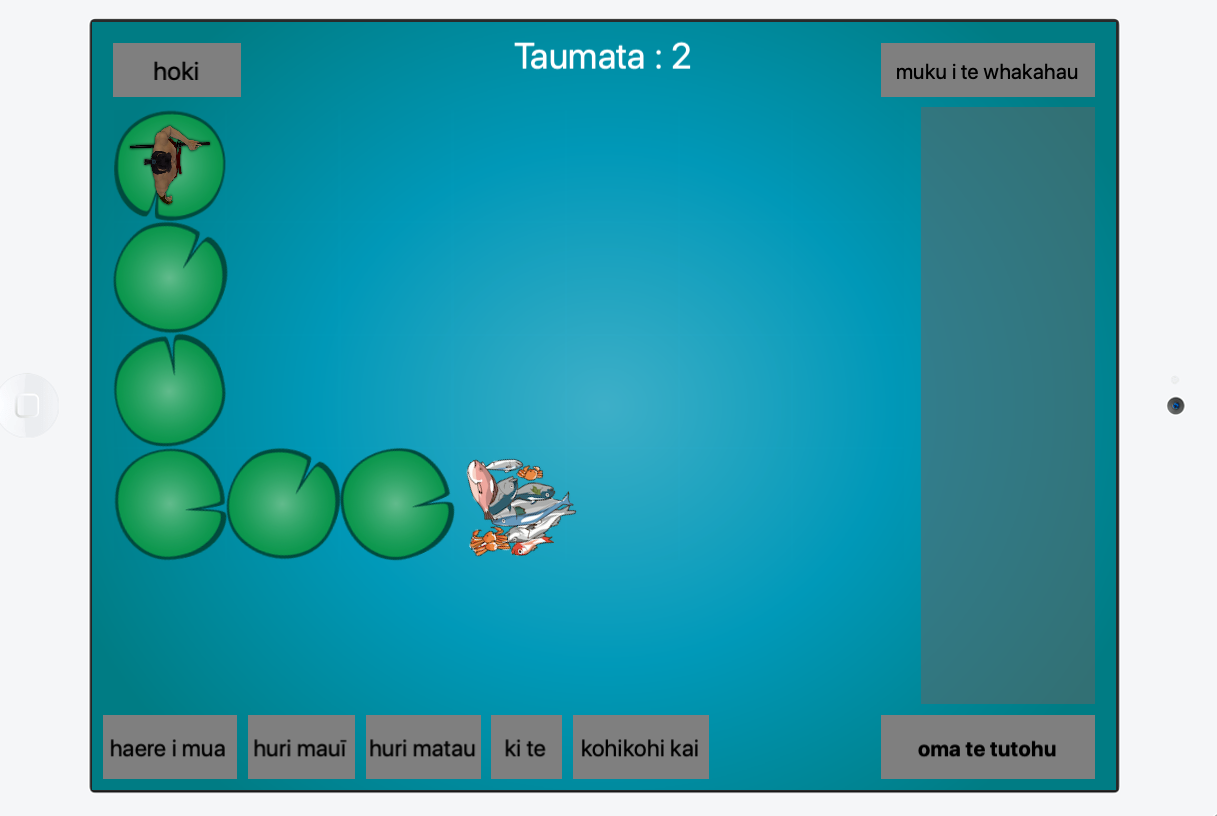
\includegraphics[width=5cm,height=3cm]{p3.png}
\column{.5\textwidth}
\centering
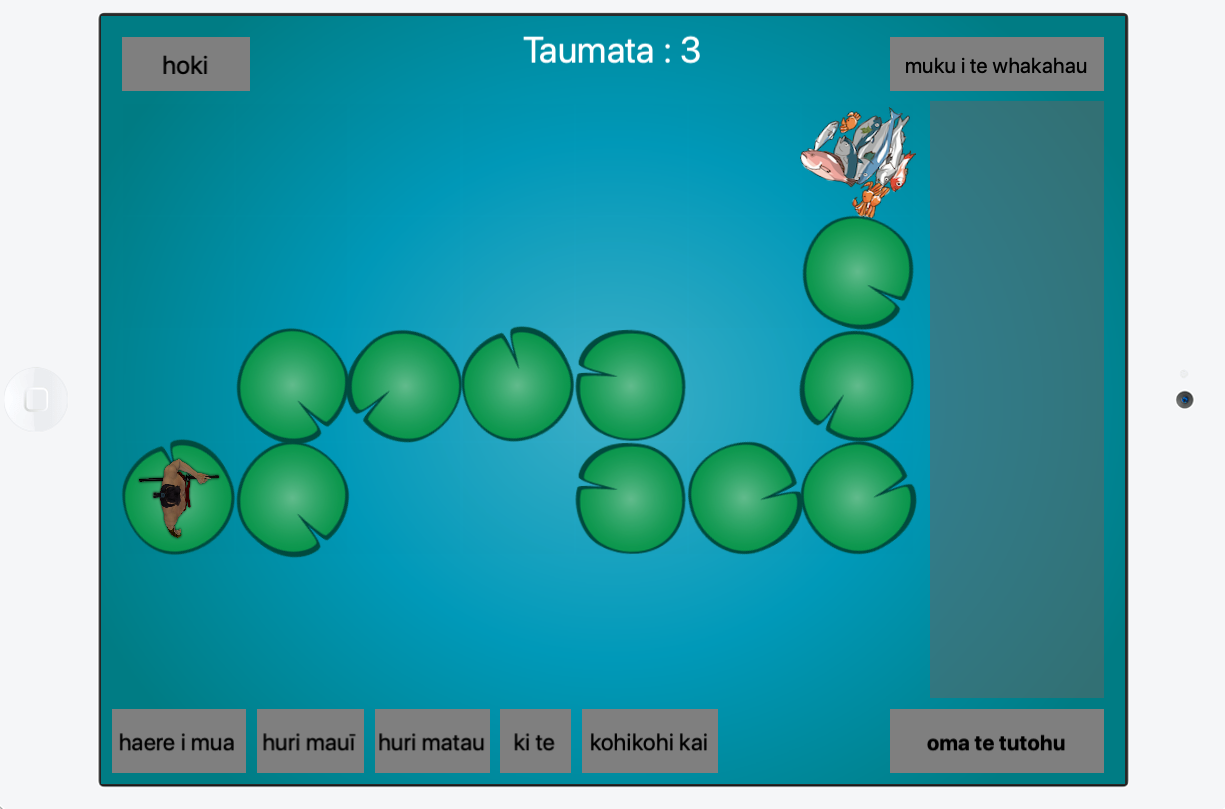
\includegraphics[width=5cm,height=4cm]{p4.png}\\
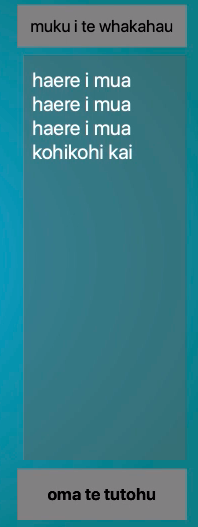
\includegraphics[width=1cm,height=3cm]{p5.png}\\
\end{columns}
\end{frame}

\section{Game Play}
\begin{frame}{Game Play}
\includemedia[
  width=0.4\linewidth,
  totalheight=0.225\linewidth,
  activate=pageopen,
  passcontext,  %show VPlayer's right-click menu
  addresource=kupe.mov,
  flashvars={
    %important: same path as in `addresource'
    source=kupe.mov
  }
]{\fbox{Click!}}{VPlayer.swf}

\end{frame}


\section{Learning CS Concepts}
\begin{frame}
\frametitle{Learning CS Concepts}

\begin{itemize}
\item  By programming the character - Kupe, the player learns basic CS concepts such as \textbf{\textit{ variables, conditionals, loops}}, among others
\newline
\item To program the character, the player presses on Kupe and this
brings up an overlay where the player can give several commands
\newline	
\item When finishing giving commands to Kupe, he will then start to move according to the commands given
\newline	
\item The player can then see how the commands give control to Kupe and he might, or might not move 	
\end{itemize}
\end{frame}

\section{Summary}
\begin{frame}
\frametitle{Summary}

\begin{itemize}
\item  Encouraging and utilizing pupil’s prior cultural knowledge and learning preferences (i.e. cultural learning styles) is a new way to learn computer programming 
\newline
\item This approach could enhance pupil's motivation and acceptance to learn computer programming concepts
\newline	
\item Integrating game-based approach would increase the student's acceptance levels and thereby encourages them to learn programming in their own intellectual style and preferences 
\newline	
\end{itemize}
\end{frame}
\ThankYouFrame

\end{document}